\documentclass[12pt,a4paper]{report}

\usepackage{graphicx}
\usepackage{amsmath}
\usepackage{hyperref}
\usepackage{booktabs}
\usepackage{listings}
\usepackage{xcolor}
\usepackage{float}
\usepackage{tikz}
\usepackage{algorithm}
\usepackage{algpseudocode}
\usepackage{changepage} % ensure this is in your preamble

\usetikzlibrary{arrows,shapes,positioning,shadows,trees,calc}

\hypersetup{
    colorlinks=true,
    linkcolor=blue,
    filecolor=magenta,
    urlcolor=cyan,
}

\lstset{
  backgroundcolor=\color{white},
  basicstyle=\footnotesize\ttfamily,
  breakatwhitespace=false,
  breaklines=true,
  captionpos=b,
  commentstyle=\color{green},
  escapeinside={\%*}{*)},
  extendedchars=true,
  frame=single,
  keepspaces=true,
  keywordstyle=\color{blue},
  language=Python,
  numbers=left,
  numbersep=5pt,
  numberstyle=\tiny\color{gray},
  rulecolor=\color{black},
  showspaces=false,
  showstringspaces=false,
  showtabs=false,
  stepnumber=1,
  stringstyle=\color{red},
  tabsize=2,
  title=\lstname
}

\title{CPU Scheduling Algorithms Simulation Project}
\author{Youness Anouar \and Abdeljalil Otman}
\date{May 2, 2025}

\begin{document}

\maketitle

\begin{abstract}
This report presents the design and implementation of a comprehensive CPU scheduling simulation project. The project includes implementations of five classic scheduling algorithms: First-Come First-Served (FCFS), Shortest Job First (SJF), Priority Scheduling, Round Robin (RR), and Priority Round Robin (PRR). The report details the design choices, implementation decisions, usage scenarios, testing methodology, and performance comparisons between the algorithms. The simulation provides an interactive visual interface for educational purposes, allowing users to understand the behavior and efficiency of different scheduling approaches.
\end{abstract}

\tableofcontents

\chapter{Introduction}
\section{Project Overview}
This project implements a CPU scheduling simulation system that demonstrates the behavior and performance of various scheduling algorithms commonly studied in operating systems courses. The simulation provides both a backend processing layer written in Python and a frontend visualization layer built with Vue.js.

\section{Objectives}
The primary objectives of this simulation project are:
\begin{itemize}
    \item To implement multiple CPU scheduling algorithms following their theoretical specifications
    \item To provide an interactive visual representation of algorithm execution
    \item To enable performance comparison between different scheduling approaches
    \item To serve as an educational tool for understanding CPU scheduling concepts
    \item To demonstrate the practical implications of theoretical scheduling principles
\end{itemize}

\section{Scope}
The simulation covers the following aspects:
\begin{itemize}
    \item Process creation with configurable attributes (arrival time, burst time, priority)
    \item Implementation of five scheduling algorithms (FCFS, SJF, Priority, Round Robin, Priority Round Robin)
    \item Visualization of process execution using Gantt charts
    \item Calculation and display of performance metrics
    \item Interactive step-by-step execution for detailed understanding
    \item Comparison tools for evaluating algorithm efficiency
\end{itemize}

\chapter{System Architecture}
\section{Overall Design}

The project follows a client-server architecture with a clear separation between the computational backend and presentation frontend:

\begin{figure}[H]
    \centering
    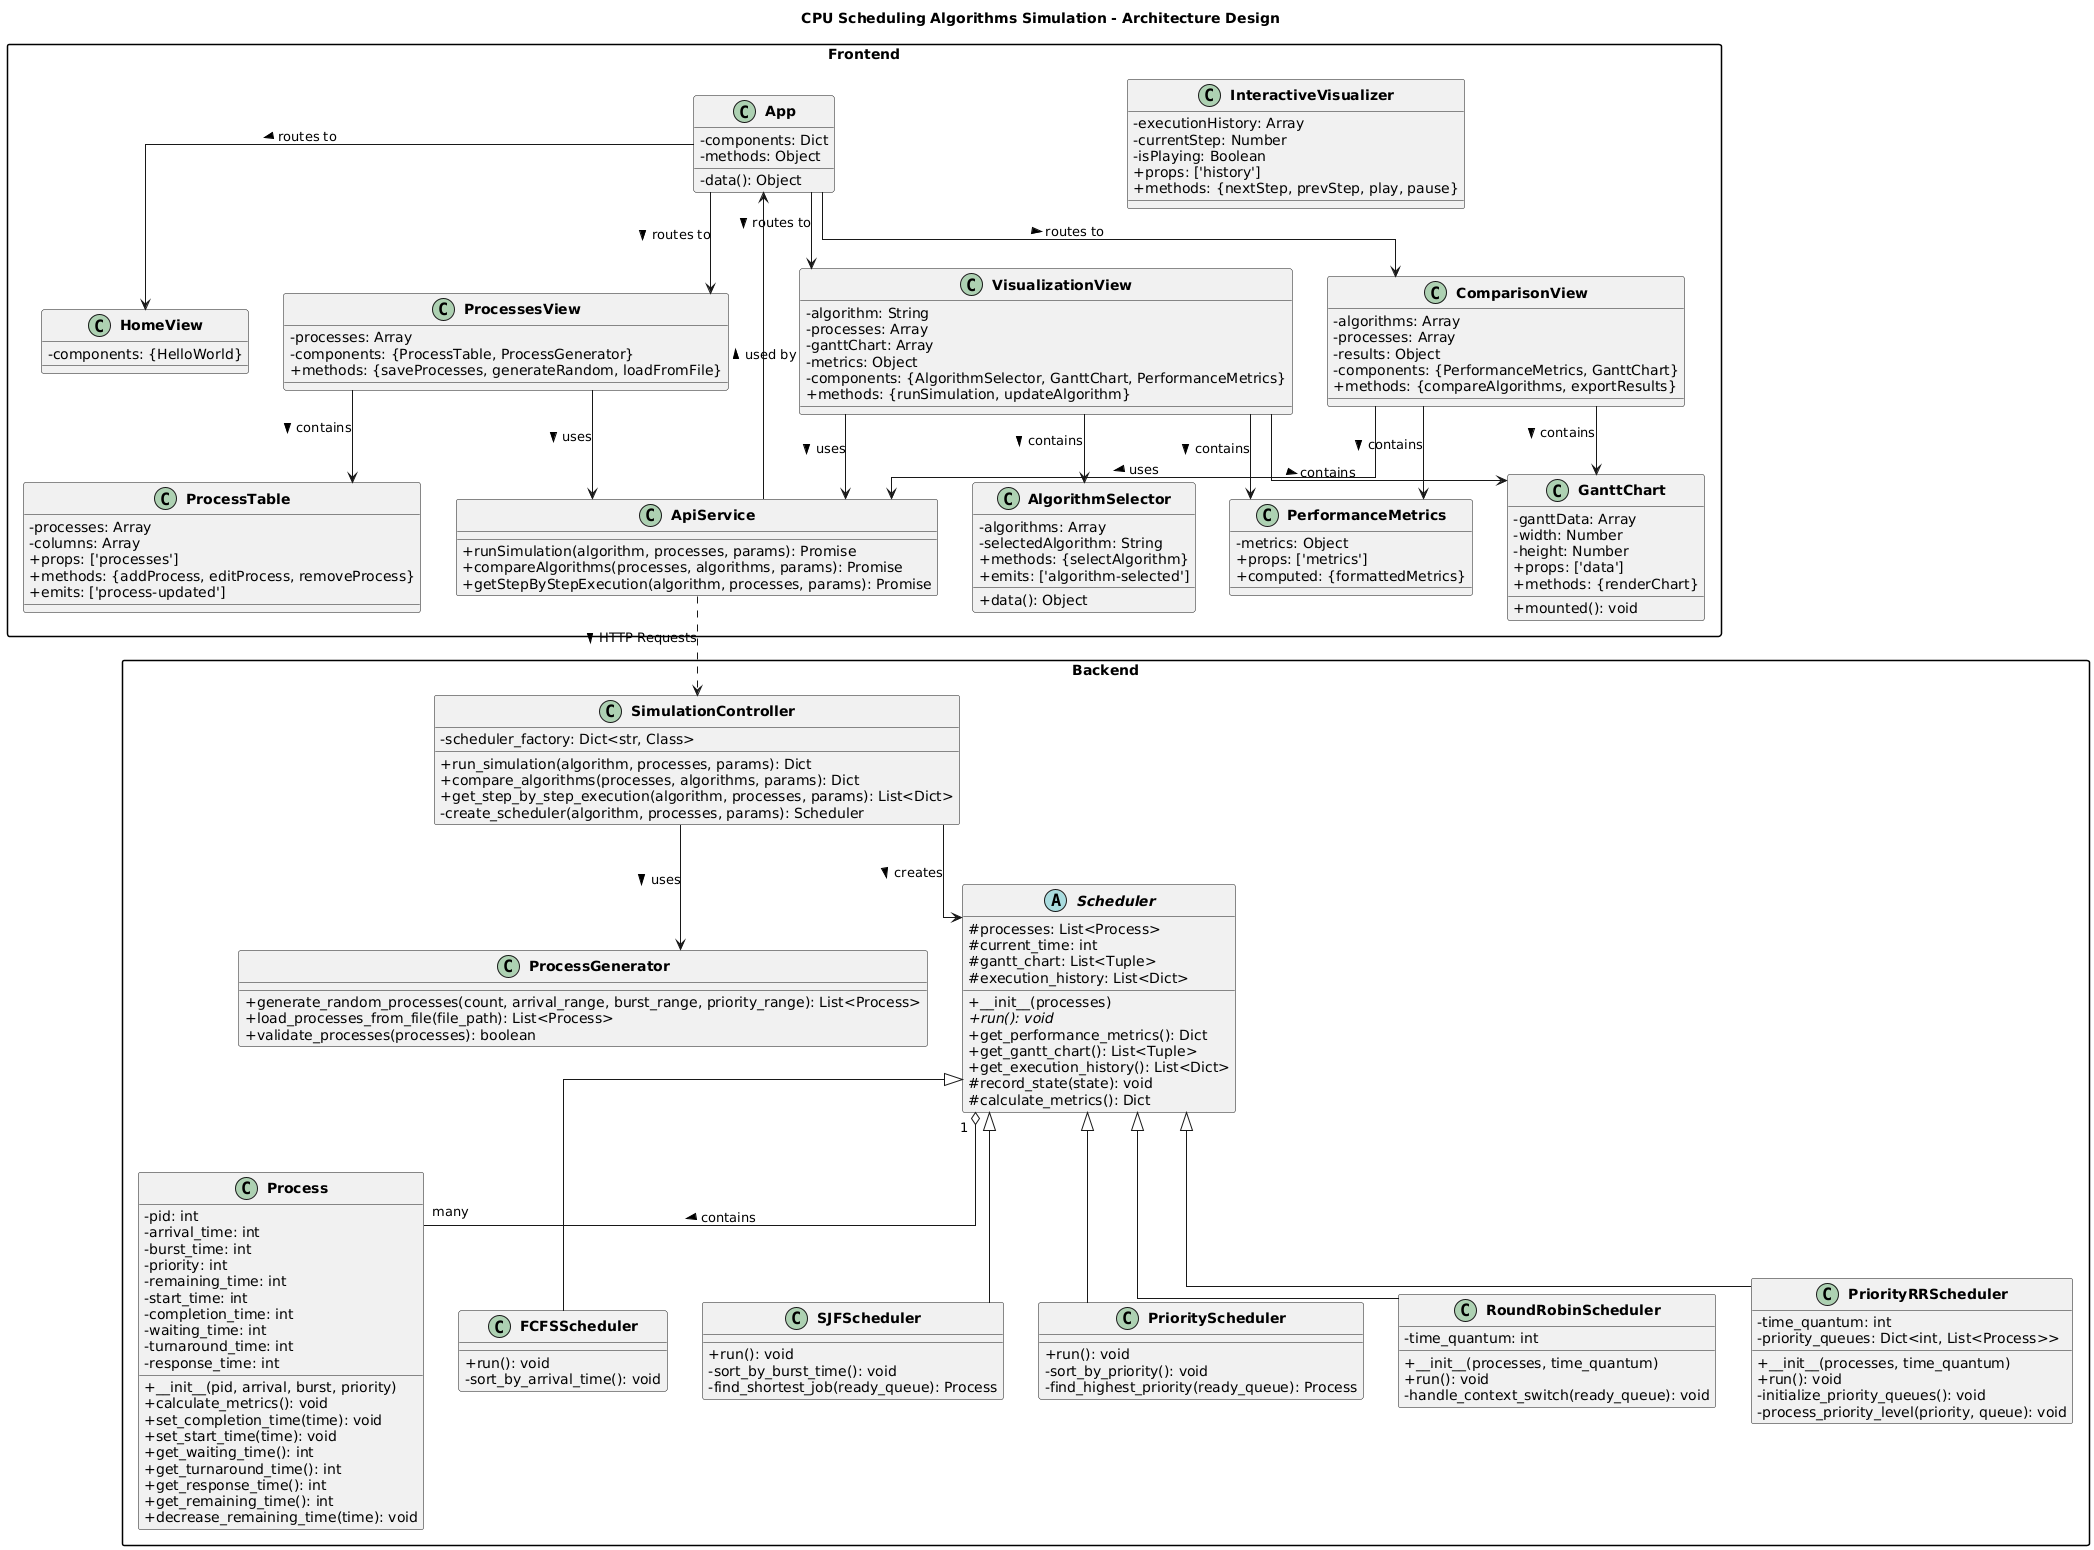
\includegraphics[width=1.0\textwidth]{classDiagram.png}
    \caption{System Architecture Class Diagram}
    \label{fig:class-diagram}
\end{figure}

% Centered, Condensed Component Interaction Diagram with Right Margin

\begin{figure}[H]
  \centering
  \begin{adjustwidth}{0pt}{2cm} % add 2cm right margin
  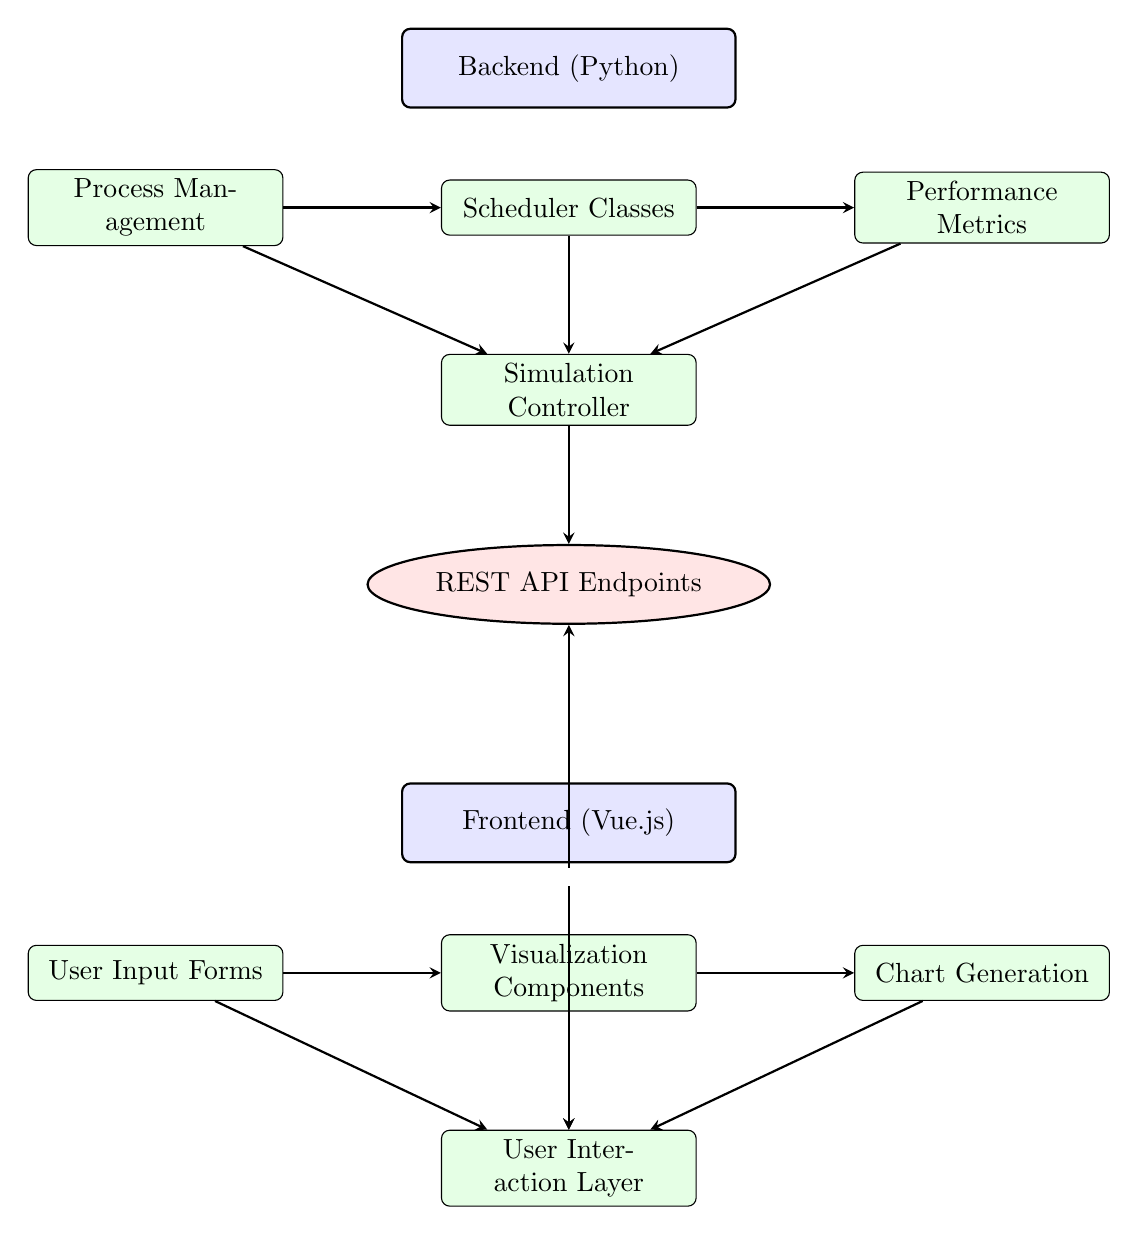
\begin{tikzpicture}[
    node distance=1cm and 2cm, % Condensed vertical and horizontal spacing
    box/.style={rectangle, draw, rounded corners=3pt, fill=blue!10, text width=4cm, minimum height=1cm, align=center, thick},
    process/.style={rectangle, draw, rounded corners=3pt, fill=green!10, text width=3cm, minimum height=0.7cm, align=center},
    arrow/.style={thick,->,>=stealth},
    comm/.style={thick,<->,>=stealth},
    cloud/.style={draw, ellipse, fill=red!10, minimum height=1cm, minimum width=3cm, align=center, thick}
  ]

    % Backend nodes (condensed)
    \node[box] (backend) {Backend (Python)};
    \node[process, below=0.9cm of backend] (scheduler) {Scheduler Classes};
    \node[process, left=of scheduler] (process) {Process Management};
    \node[process, right=of scheduler] (metrics) {Performance Metrics};
    \node[process, below=1.5cm of scheduler] (controller) {Simulation Controller};
    \node[cloud, below=1.5cm of controller] (api) {REST API Endpoints};

    % Frontend nodes (condensed)
    \node[box, below=2cm of api] (frontend) {Frontend (Vue.js)};
    \node[process, below=0.9cm of frontend] (visu) {Visualization Components};
    \node[process, left=of visu] (forms) {User Input Forms};
    \node[process, right=of visu] (charts) {Chart Generation};
    \node[process, below=1.5cm of visu] (interaction) {User Interaction Layer};

    % Backend connections
    \draw[arrow] (process) -- (scheduler);
    \draw[arrow] (scheduler) -- (metrics);
    \draw[arrow] (process) -- (controller);
    \draw[arrow] (scheduler) -- (controller);
    \draw[arrow] (metrics) -- (controller);
    \draw[arrow] (controller) -- (api);

    % Frontend connections
    \draw[arrow] (forms) -- (visu);
    \draw[arrow] (visu) -- (charts);
    \draw[arrow] (forms) -- (interaction);
    \draw[arrow] (visu) -- (interaction);
    \draw[arrow] (charts) -- (interaction);

    % Backend-Frontend communication
    \draw[comm] (api) -- node[midway, fill=white, font=\small] {} (interaction);

  \end{tikzpicture}
  \end{adjustwidth}
  \caption{Condensed Component Interaction between Frontend and Backend}
  \label{fig:component-interaction}
\end{figure}


This diagram illustrates the interaction between the system components. The backend Python modules handle the computation and simulation logic, while the frontend Vue.js components manage user interaction and visualization. Communication between the two layers occurs through REST API endpoints using HTTP requests with JSON payloads.

\section{Backend Architecture}
The backend is implemented in Python and follows object-oriented design principles. It consists of:
\begin{itemize}
    \item Core classes for process representation and management
    \item Abstract scheduler class defining common functionality
    \item Concrete scheduler implementations for each algorithm
    \item Controller class managing the simulation flow
    \item API endpoints for frontend communication
\end{itemize}

\section{Frontend Architecture}
The frontend is built using Vue.js and provides:
\begin{itemize}
    \item Responsive user interface for simulation interaction
    \item Process creation and management components
    \item Algorithm selection and parameter configuration
    \item Visualization components (Gantt charts, timelines)
    \item Performance metrics displays and comparison tools
\end{itemize}

\chapter{Design Choices}

\section{Object-Oriented Design}
We adopted an object-oriented approach for the scheduling algorithms, using the Strategy pattern through an abstract Scheduler base class with concrete implementations for each algorithm. This design:
\begin{itemize}
    \item Provides a uniform interface for all scheduling algorithms
    \item Facilitates adding new algorithms without modifying existing code
    \item Enables reuse of common functionality across algorithms
    \item Ensures consistent handling of processes and metrics
\end{itemize}

\section{Separation of Concerns}
The system separates process management, scheduling logic, and visualization:
\begin{itemize}
    \item Process class manages individual process attributes and state
    \item Scheduler classes focus exclusively on algorithm implementation
    \item Controller class coordinates execution and result collection
    \item Frontend components handle user interaction and visualization
\end{itemize}

\section{State Tracking and Simulation History}
To enable step-by-step visualization, we implemented a comprehensive state tracking mechanism:
\begin{itemize}
    \item Each algorithm records its state at significant execution steps
    \item States include ready queue contents, running process, and time information
    \item History can be replayed for educational purposes
    \item Interactive visualization uses this data for detailed exploration
\end{itemize}

\chapter{Implementation Details}

\section{Process Representation}
Each process is represented by the \texttt{Process} class with the following attributes:
\begin{itemize}
    \item Process ID: Unique identifier
    \item Arrival Time: When the process enters the system
    \item Burst Time: CPU time required for execution
    \item Priority: Importance value (lower value means higher priority)
    \item State variables: Remaining time, start time, completion time, etc.
\end{itemize}

Mathematically, a process $P_i$ can be represented as:
\begin{align}
P_i = (id_i, arrival_i, burst_i, priority_i, remaining_i, start_i, completion_i)
\end{align}

where:
\begin{align}
waiting_i &= completion_i - arrival_i - burst_i\\
turnaround_i &= completion_i - arrival_i\\
response_i &= start_i - arrival_i
\end{align}

\section{Scheduler Base Class}
The abstract \texttt{Scheduler} class provides common functionality:
\begin{itemize}
    \item Process list management
    \item Time tracking
    \item Gantt chart creation
    \item Performance metric calculations
    \item Simulation state recording
\end{itemize}

\section{Algorithm Implementations}

\subsection{First-Come First-Served (FCFS)}
FCFS executes processes in the order they arrive:
\begin{itemize}
    \item Non-preemptive scheduling
    \item Sorts processes by arrival time
    \item Simple implementation with a FIFO queue
    \item Records state changes when processes arrive and complete
\end{itemize}

Formally, FCFS scheduling can be defined as:
\begin{align}
\text{Given processes } P = \{P_1, P_2, \ldots, P_n\}\\
\text{Order by } arrival_i \text{ such that }\\
\forall i,j \in \{1,2,\ldots,n\}, i < j \implies arrival_i \leq arrival_j
\end{align}

\begin{algorithm}[H]
\caption{FCFS Algorithm}
\begin{algorithmic}[1]
    \State Sort processes by arrival time
    \ForEach{process in sorted order}
        \State Execute process until completion
    \EndFor
\end{algorithmic}
\end{algorithm}

\subsection{Shortest Job First (SJF)}
SJF executes the process with the shortest burst time first:
\begin{itemize}
    \item Non-preemptive implementation
    \item Maintains a priority queue sorted by burst time
    \item Records state changes at process selection and completion
\end{itemize}

Let $R(t)$ be the set of ready processes at time $t$. SJF selects process $P_i$ such that:
\begin{align}
P_i \in R(t) \wedge \forall P_j \in R(t): burst_i \leq burst_j
\end{align}

\begin{algorithm}[H]
\caption{SJF Algorithm}
\begin{algorithmic}[1]
    \While{not all processes finished}
        \State Select process with smallest burst time in $R(t)$
        \State Execute until completion
    \EndWhile
\end{algorithmic}
\end{algorithm}

\subsection{Priority Scheduling}
Priority scheduling executes processes based on priority value:
\begin{itemize}
    \item Non-preemptive implementation
    \item Maintains a priority queue sorted by priority value
    \item Lower numerical value indicates higher priority
    \item Records state changes at priority-based selection points
\end{itemize}

Let $R(t)$ be the set of ready processes at time $t$. Priority Scheduling selects process $P_i$ such that:
\begin{align}
P_i \in R(t) \wedge \forall P_j \in R(t): priority_i \leq priority_j
\end{align}

\begin{algorithm}[H]
\caption{Priority Scheduling Algorithm}
\begin{algorithmic}[1]
    \While{not all processes finished}
        \State Select process with highest priority in $R(t)$
        \State Execute until completion
    \EndWhile
\end{algorithmic}
\end{algorithm}

\subsection{Round Robin (RR)}
Round Robin allocates a fixed time quantum $q$ to each process:
\begin{itemize}
    \item Preemptive scheduling with configurable time quantum
    \item Circular queue implementation
    \item Records state changes at context switches and quantum expirations
    \item Tracks remaining burst time for each process
\end{itemize}

For each time slice of length $q$:
\begin{align}
execution\_time_i &= \min(remaining_i, q)\\
remaining_i &= remaining_i - execution\_time_i
\end{align}

If $remaining_i > 0$, the process is placed back in the ready queue.

\begin{algorithm}[H]
\caption{Round Robin Algorithm}
\begin{algorithmic}[1]
    \While{not all processes finished}
        \ForEach{process in ready queue}
            \State Execute for up to $q$ time units
            \If{burst not finished}
                \State Put process back in queue with updated remaining time
            \EndIf
        \EndFor
    \EndWhile
\end{algorithmic}
\end{algorithm}

\subsection{Priority Round Robin (PRR)}
Priority Round Robin combines priority scheduling with round robin:
\begin{itemize}
    \item Processes are grouped by priority level
    \item Round Robin is applied within each priority group
    \item Multiple queue implementation with highest priority served first
    \item Records detailed state of all priority queues
\end{itemize}

PRR can be formally described as:
\begin{align}
\text{Let } Q_p = \{P_i \in R(t) \mid priority_i = p\}\\
\text{Execute processes in } Q_{p_{min}} \text{ using Round Robin with quantum } q\\
\text{If } Q_{p_{min}} = \emptyset \text{, move to } Q_{p_{min}+1}
\end{align}

\begin{algorithm}[H]
\caption{Priority Round Robin Algorithm}
\begin{algorithmic}[1]
    \While{not all processes finished}
        \For{priority level from highest to lowest}
            \While{there are processes in $Q_p$}
                \State Execute each process using RR with quantum $q$
            \EndWhile
        \EndFor
    \EndWhile
\end{algorithmic}
\end{algorithm}


\section{Performance Metrics Calculation}
The simulation calculates standard CPU scheduling performance metrics:

\begin{align}
\text{Average Waiting Time} &= \frac{1}{n} \sum_{i=1}^{n} waiting_i\\
\text{Average Turnaround Time} &= \frac{1}{n} \sum_{i=1}^{n} turnaround_i\\
\text{Average Response Time} &= \frac{1}{n} \sum_{i=1}^{n} response_i\\
\text{CPU Utilization} &= \frac{\sum_{i=1}^{n} burst_i}{\max_i(completion_i) - \min_i(arrival_i)} \times 100\%\\
\text{Throughput} &= \frac{n}{\max_i(completion_i) - \min_i(arrival_i)}
\end{align}

Where $n$ is the total number of processes.

\section{Visualization Components}
The frontend includes specialized visualization components:
\begin{itemize}
    \item Gantt Chart: Shows process execution timeline
    \item Process Table: Displays all process attributes and calculated metrics
    \item Interactive Visualizer: Step-by-step algorithm execution
    \item Performance Metrics Display: Shows calculated metrics in real-time
\end{itemize}

\chapter{Usage Scenarios}

\section{Educational Use Case}
The primary use case is educational, allowing students to:
\begin{itemize}
    \item Explore scheduling algorithm behavior with different process sets
    \item Observe how algorithm selection affects performance metrics
    \item Understand trade-offs between different scheduling approaches
    \item Learn through interactive visualization and step-by-step execution
\end{itemize}

\section{Process Creation}
Users can create processes through:
\begin{itemize}
    \item Manual process specification (ID, arrival time, burst time, priority)
    \item Random process generation with configurable parameters
    \item File upload (CSV or JSON format)
\end{itemize}

\section{Algorithm Visualization}
The system supports two visualization modes:
\begin{itemize}
    \item Basic mode: Shows complete execution results and metrics
    \item Interactive mode: Allows stepping through the algorithm execution
\end{itemize}

\section{Performance Comparison}
Users can compare algorithms by:
\begin{itemize}
    \item Running multiple algorithms on the same process set
    \item Viewing side-by-side metric comparisons
    \item Analyzing Gantt charts to understand execution differences
    \item Exploring how time quantum affects Round Robin performance
\end{itemize}

\chapter{Testing Methodology}

\section{Unit Testing}
Each component was tested individually:
\begin{itemize}
    \item Process class methods for correct timing calculations
    \item Individual scheduler algorithm implementations
    \item Performance metric calculation accuracy
\end{itemize}

\section{Integration Testing}
Integration tests verified the interaction between components:
\begin{itemize}
    \item Controller integration with scheduler implementations
    \item API endpoint functionality with frontend requests
    \item End-to-end simulation flow
\end{itemize}

\section{Test Cases}
Standard test cases included:

\subsection{Test Case 1: Basic Process Set}
\begin{tabular}{|c|c|c|c|}
\hline
Process ID & Arrival Time & Burst Time & Priority \\
\hline
P1 & 0 & 5 & 3 \\
P2 & 1 & 3 & 1 \\
P3 & 2 & 8 & 2 \\
P4 & 3 & 2 & 4 \\
\hline
\end{tabular}

\subsection{Test Case 2: Simultaneous Arrival}
\begin{tabular}{|c|c|c|c|}
\hline
Process ID & Arrival Time & Burst Time & Priority \\
\hline
P1 & 0 & 6 & 3 \\
P2 & 0 & 4 & 1 \\
P3 & 0 & 3 & 2 \\
P4 & 0 & 5 & 4 \\
\hline
\end{tabular}

\subsection{Test Case 3: Priority Evaluation}
\begin{tabular}{|c|c|c|c|}
\hline
Process ID & Arrival Time & Burst Time & Priority \\
\hline
P1 & 0 & 5 & 4 \\
P2 & 1 & 7 & 2 \\
P3 & 2 & 3 & 1 \\
P4 & 3 & 4 & 3 \\
\hline
\end{tabular}

\subsection{Test Case 4: Round Robin Evaluation}
\begin{tabular}{|c|c|c|}
\hline
Process ID & Arrival Time & Burst Time \\
\hline
P1 & 0 & 10 \\
P2 & 0 & 5 \\
P3 & 0 & 8 \\
\hline
\end{tabular}
Tested with time quantum values: 1, 2, 4, and 8

\section{Edge Cases}
We tested the following edge cases:
\begin{itemize}
    \item Empty process list
    \item Single process execution
    \item Processes with zero burst time
    \item Late-arriving high-priority processes
    \item Very large process sets (>100 processes)
    \item Extremely small and large time quantum values
\end{itemize}

\chapter{Performance Analysis}

\section{Comparison Methodology}
To compare algorithm performance, we:
\begin{itemize}
    \item Used identical process sets across all algorithms
    \item Varied process characteristics (arrival patterns, burst times, priorities)
    \item Measured standard performance metrics
    \item Evaluated impact of time quantum on Round Robin variants
\end{itemize}

\section{Results}
\subsection{Average Waiting Time}
SJF generally provided the lowest average waiting time, as expected from theoretical analysis. FCFS performed worst with varying burst times, while Round Robin's performance depended heavily on time quantum selection.

For a set of $n$ processes, the theoretical lower bound on average waiting time is achieved by SJF and can be approximated as:
\begin{align}
\text{AWT}_{SJF} \approx \frac{\sum_{i=1}^{n-1} \sum_{j=i+1}^{n} \min(burst_i, burst_j)}{n}
\end{align}

\subsection{Average Turnaround Time}
Similar to waiting time, SJF typically showed the best turnaround time. Priority scheduling performed well when high-priority processes had short burst times.

\subsection{CPU Utilization}
All non-preemptive algorithms (FCFS, SJF, Priority) showed similar CPU utilization. Round Robin variants had slightly lower utilization due to context switching overhead, which can be modeled as:
\begin{align}
\text{Utilization}_{RR} \approx \frac{\sum_{i=1}^{n} burst_i}{\sum_{i=1}^{n} burst_i + k \times \text{context\_switch\_time}}
\end{align}
where $k$ is the number of context switches.

\subsection{Time Quantum Effects}
For Round Robin and Priority Round Robin:

The average waiting time in Round Robin can be approximately modeled as a function of time quantum $q$:
\begin{align}
\text{AWT}_{RR}(q) \approx \text{AWT}_{FCFS} - \frac{q}{2} \times \frac{n-1}{n} \times (1 - \frac{1}{\bar{b}/q})
\end{align}
where $\bar{b}$ is the average burst time.

\begin{itemize}
    \item Small time quantum ($q \ll \bar{b}$): Increased responsiveness but reduced efficiency due to context switching
    \item Large time quantum ($q \gg \bar{b}$): Improved efficiency but reduced fairness, approaching FCFS behavior
    \item Optimal time quantum: Empirically found to be around $q \approx \bar{b}/2$
\end{itemize}

\section{Algorithm Strengths and Weaknesses}
\subsection{FCFS}
\begin{itemize}
    \item Strengths: Simplicity, fairness in arrival order, no starvation
    \item Weaknesses: Convoy effect, poor average waiting time with varying burst times
\end{itemize}

\subsection{SJF}
\begin{itemize}
    \item Strengths: Optimal average waiting time, good for batch systems
    \item Weaknesses: Potential starvation of longer jobs, requires known burst times
\end{itemize}

\subsection{Priority Scheduling}
\begin{itemize}
    \item Strengths: Importance-based execution, good for systems with critical tasks
    \item Weaknesses: Starvation of low-priority processes, priority inversion problems
\end{itemize}

\subsection{Round Robin}
\begin{itemize}
    \item Strengths: Fair CPU distribution, good response time, no starvation
    \item Weaknesses: Higher context switching overhead, performance sensitive to time quantum
\end{itemize}

\subsection{Priority Round Robin}
\begin{itemize}
    \item Strengths: Combines benefits of Priority and Round Robin, flexible
    \item Weaknesses: Complex implementation, requires careful parameter tuning
\end{itemize}

\chapter{Conclusion}
\section{Summary of Findings}
Our simulation confirmed theoretical principles of CPU scheduling:
\begin{itemize}
    \item SJF provides optimal average waiting time but is impractical in real systems
    \item FCFS is simple but can lead to poor performance with mixed process types
    \item Priority scheduling handles different process importance but risks starvation
    \item Round Robin provides fairness and responsiveness at the cost of efficiency
    \item Priority Round Robin offers a good compromise for many scenarios
\end{itemize}

The mathematical analysis revealed that:
\begin{align}
\text{AWT}_{SJF} \leq \text{AWT}_{Priority} \leq \text{AWT}_{FCFS}
\end{align}

And for Round Robin, the relation between time quantum $q$ and performance follows:
\begin{align}
\lim_{q \to \infty} \text{AWT}_{RR}(q) &= \text{AWT}_{FCFS}\\
\lim_{q \to 0} \text{AWT}_{RR}(q) &= \infty \text{ (due to context switching overhead)}
\end{align}

\section{Future Improvements}
Potential enhancements for the simulation include:
\begin{itemize}
    \item Implementation of additional algorithms (Multilevel Feedback Queue with decay function $\alpha(t) = \frac{1}{1+t}$)
    \item Stochastic process models with burst time distribution $B \sim N(\mu, \sigma^2)$
    \item Real-time visualization with dynamic parameter adjustment
    \item Machine learning models for predicting optimal scheduling parameters
\end{itemize}

\section{Final Thoughts}
This simulation demonstrates the fundamental trade-offs in CPU scheduling algorithms, confirming the theoretical time complexity and performance characteristics. No algorithm provides an optimal solution across all scenarios, making scheduling policy selection context-dependent.

\end{document}